\section{Experiments}
\label{sec:results}

\begin{table*}[h]
\begin{small}
\centering
\begin{tabular}{cccccccc}
\hline
\multirow{3}{2cm}{\centering Score Function}& \multirow{3}{2cm}{Algorithm} & \multicolumn{2}{c}{FB15K-237} & \multicolumn{2}{c}{WN18} & \multicolumn{2}{c}{WN18RR} \\
& & Hit@10 & \multirow{2}{1cm}{\centering MRR} & Hit@10 & \multirow{2}{1cm}{\centering MRR} & Hit@10 & \multirow{2}{1cm}{\centering MRR} \\ 
& & (\%) & & (\%) & & (\%) & \\
\hline
% TransE --------------------------------------------------
\multirow{5}{1.5cm}{\centering TransE} & KBGAN \cite{cai2017kbgan} & 46.59 & 0.2926 & 94.80 & 0.6606 & 45.39 & 0.1808 \\
& NSCaching \cite{zhang2019nscaching} & 47.64 & \textbf{0.2993} & 94.63 & 0.7818$^\dagger$ & 47.83 & 0.2002\\
& Uniform \cite{sun2019rotate} & 48.03$^\dagger$ & 0.2927 & \textbf{95.53} & 0.6085 & 49.63$^\dagger$ & 0.2022$^\dagger$ \\
& Uniform SANS (ours) & \textbf{48.35} & 0.2962$^\dagger$ & 95.09$^\dagger$ & \textbf{0.8228} & \textbf{51.15} & \textbf{0.2254} \\
& $\Delta$ & \cellcolor{celadon}+0.32 & \cellcolor{mistyrose}-0.0031 & \cellcolor{mistyrose}-0.44 &	\cellcolor{celadon}+0.041 & \cellcolor{celadon}+1.52	& \cellcolor{celadon}+0.0232 \\
\hline
% DistMult --------------------------------------------------
\multirow{5}{1.5cm}{\centering DistMult} & KBGAN & 39.91 & 0.2272 & 93.08 & 0.7275 & 44.32 & 0.3849 \\
& NSCaching & \textbf{45.56} & \textbf{0.2834} & \textbf{93.74} & \textbf{0.8306} & 45.80$^\dagger$ & \textbf{0.4148} \\
& Uniform & 40.26 & 0.2537 & 81.39  & 0.4689 & \textbf{52.86} & 0.3938$^\dagger$ \\
& Uniform SANS (ours) & 41.00$^\dagger$ & 0.2595$^\dagger$ & 93.19$^\dagger$ & 0.7553$^\dagger$ & 44.74 & 0.4025 \\
& $\Delta$ & \cellcolor{mistyrose}-4.56 & \cellcolor{mistyrose}-0.0239 & \cellcolor{mistyrose}-0.55 & \cellcolor{mistyrose}-0.0753 &	\cellcolor{mistyrose}-8.12 & \cellcolor{mistyrose}-0.0123 \\
\hline
% RotatE --------------------------------------------------
\multirow{3}{1cm}{\centering RotatE} & Uniform & 47.85$^\dagger$ & 0.2946$^\dagger$ & \textbf{96.09} & 0.9474$^\dagger$ & \textbf{56.51} & 0.4711$^\dagger$ \\
& Uniform SANS (ours) & \textbf{48.22 }& \textbf{0.2985} & 95.97$^\dagger$ & \textbf{0.9499} & 55.76$^\dagger$ & \textbf{0.4769} \\
& $\Delta$ & \cellcolor{celadon}+0.37 & \cellcolor{celadon}+0.0039 & \cellcolor{mistyrose}-0.12 & \cellcolor{celadon}+0.0025 & \cellcolor{mistyrose}-0.75 & \cellcolor{celadon}+0.0058\\
\hline
\end{tabular}
\caption{Comparison of different negative sampling algorithms. Bold and $\dagger$ numbers represent best and second-best performance respectively. Results for KBGAN and NSCaching are taken from \cite{zhang2019nscaching}.
}
\label{tab:unisota_comp}
\end{small}
\end{table*}
% ------------------------------------------------------------
% ------------------------------------------------------------% ------------------------------------------------------------
% ---- BACKUP
\cut{
\begin{table*}[h]
\begin{small}
\centering
\begin{tabular}{cccccccc}
\hline
\multirow{3}{2cm}{\centering Score Function}& \multirow{3}{2cm}{Algorithm} & \multicolumn{2}{c}{FB15K-237} & \multicolumn{2}{c}{WN18} & \multicolumn{2}{c}{WN18RR} \\
& & Hit@10 & \multirow{2}{1cm}{\centering MRR} & Hit@10 & \multirow{2}{1cm}{\centering MRR} & Hit@10 & \multirow{2}{1cm}{\centering MRR} \\ 
& & (\%) & & (\%) & & (\%) & \\
\hline
% TransE --------------------------------------------------
\multirow{5}{1.5cm}{\centering TransE} & KBGAN \cite{cai2017kbgan} & 46.59 & 0.2926 & 94.80 & 0.6606 & 45.39 & 0.1808 \\
& NSCaching \cite{zhang2019nscaching} & 47.64 & \textbf{0.2993} & 94.63 & 0.7818$^\dagger$ & 47.83 & 0.2002\\
& Uniform \cite{sun2019rotate} & 48.03$^\dagger$ & 0.2927 & \textbf{95.53} & 0.6085 & 49.63$^\dagger$ & 0.2022$^\dagger$ \\
& Uniform SANS (ours) & \textbf{48.35} & 0.2962$^\dagger$ & 95.09$^\dagger$ & \textbf{0.8228} & \textbf{51.15} & \textbf{0.2254} \\
& $\Delta$ & \cellcolor{palegreen}+0.32 & \cellcolor{palegreen}+0.0035 & \cellcolor{mistyrose}-0.44 &	\cellcolor{palegreen}+0.2143 & \cellcolor{palegreen}+1.52	& \cellcolor{palegreen}+0.0232 \\
\hline
% DistMult --------------------------------------------------
\multirow{5}{1.5cm}{\centering DistMult} & KBGAN & 39.91 & 0.2272 & 93.08 & 0.7275 & 44.32 & 0.3849 \\
& NSCaching & \textbf{45.56} & \textbf{0.2834} & \textbf{93.74} & \textbf{0.8306} & 45.80$^\dagger$ & \textbf{0.4148} \\
& Uniform & 40.26 & 0.2537 & 81.39  & 0.4689 & \textbf{52.86} & 0.3938$^\dagger$ \\
& Uniform SANS (ours) & 41.00$^\dagger$ & 0.2595$^\dagger$ & 93.19$^\dagger$ & 0.7553$^\dagger$ & 44.74 & 0.4025 \\
& $\Delta$ & \cellcolor{palegreen}+0.7400 & \cellcolor{palegreen}+0.0058 & \cellcolor{palegreen}+11.80 & \cellcolor{palegreen}+0.2864 &	\cellcolor{mistyrose}-8.12 & \cellcolor{palegreen}+0.0087 \\
\hline
% RotatE --------------------------------------------------
\multirow{3}{1cm}{\centering RotatE} & Uniform & 47.85$^\dagger$ & 0.2946$^\dagger$ & \textbf{96.09} & 0.9474$^\dagger$ & \textbf{56.51} & 0.4711$^\dagger$ \\
& Uniform SANS (ours) & \textbf{48.22 }& \textbf{0.2985} & 95.97$^\dagger$ & \textbf{0.9499} & 55.76$^\dagger$ & \textbf{0.4769} \\
& $\Delta$ & \cellcolor{palegreen}+0.37 & \cellcolor{palegreen}+0.0039 & \cellcolor{mistyrose}-0.12 & \cellcolor{palegreen}+0.0025 & \cellcolor{mistyrose}-0.75 & \cellcolor{palegreen}+0.0058\\
\hline
\end{tabular}
\caption{Comparison of different negative sampling algorithms. Bold and $\dagger$ numbers represent best and second-best performance respectively. Results for KBGAN and NSCaching are taken from \cite{zhang2019nscaching}.
}
\label{tab:unisota_comp}
\end{small}
\end{table*}}
% RESULTS TABLE 2 START
\begin{table*}[h]
\begin{small}
\centering
\begin{tabular}{cccccccc}
\hline
\multirow{3}{2cm}{\centering Score Function}& \multirow{3}{2cm}{Algorithm} & \multicolumn{2}{c}{FB15K-237} & \multicolumn{2}{c}{WN18} & \multicolumn{2}{c}{WN18RR} \\
& & Hit@10 & \multirow{2}{1cm}{\centering MRR} & Hit@10 & \multirow{2}{1cm}{\centering MRR} & Hit@10 & \multirow{2}{1cm}{\centering MRR} \\ 
& & (\%) & & (\%) & & (\%) & \\
\hline
% TransE --------------------------------------------------
\multirow{3}{1.5cm}{\centering TransE} & Self-Adv. \cite{sun2019rotate} & \textbf{52.73} & \textbf{0.3296} & \textbf{92.02} & \textbf{0.7722} & 52.78 & 0.2232 \\
& Self-Adv. SANS (ours) & 52.03 & 0.3265 & 84.06 & 0.7136 & \textbf{53.21} & \textbf{0.2249} \\
& $\Delta$ & \cellcolor{mistyrose}-0.7 & \cellcolor{mistyrose}-0.0031 & \cellcolor{mistyrose}-7.96 &	\cellcolor{mistyrose} -0.0586 & \cellcolor{palegreen}+0.43 & \cellcolor{palegreen}+0.0017 \\
\hline
% DistMult --------------------------------------------------
\multirow{3}{1.5cm}{\centering DistMult} & Self-Adv. & 48.41 & 0.3091 & 92.94  & 0.6837 & \textbf{53.80} & \textbf{0.4399} \\
& Self-Adv. SANS (ours) & \textbf{48.68} & \textbf{0.3100} & \textbf{93.04} & \textbf{0.7561} & 38.70 & 0.3684 \\
& $\Delta$ & \cellcolor{palegreen}+0.27 & \cellcolor{palegreen} +0.0009 & \cellcolor{palegreen}+0.1 &	\cellcolor{palegreen}+0.0724 & \cellcolor{mistyrose} -15.10 & \cellcolor{mistyrose}-0.0715 \\
\hline
% RotatE --------------------------------------------------
\multirow{3}{1cm}{\centering RotatE} & Self-Adv. & 53.03 & \textbf{0.3362} & \textbf{96.05}& \textbf{0.9498} & \textbf{57.29} & \textbf{0.4760} \\
& Self-Adv. SANS (ours) & \textbf{53.12} & 0.3358 & 95.85 & 0.9494 & 57.12 & 0.4745 \\
& $\Delta$ & \cellcolor{palegreen}+0.09 & \cellcolor{mistyrose}-0.0004 &  \cellcolor{mistyrose}-0.2 & \cellcolor{mistyrose}-0.0004	& \cellcolor{mistyrose}-0.17	& \cellcolor{mistyrose}-0.0015 \\
\hline
\end{tabular}
\caption{Comparison of the Self-Adversarial negative sampling technique with our Self-Adversarial SANS. 
}
\label{tab:comp_adv}
\end{small}
\end{table*}
% RESULTS TABLE 2 END

We investigate the application of SANS based negatives to train KG's embedding models based on  the TransE, DistMult, and RotatE models for the task of KG completion. We evaluate our proposed approach on standard benchmarks consisting of a variant of FreeBase in FB15K-237 \cite{bollacker2008freebase}, WN18 and WN18RR \cite{miller1995wordnet}. From our experiments we seek to answer the following questions: 
\begin{itemize}
    \item[\textbf{(Q1)}] \textbf{Hard Negatives: Can we sample hard negatives purely using graph structure?} 
    \item[\textbf{(Q2)}] \textbf{Can we combine graph structure with other SOTA negative samplers ?} 
    \item[\textbf{(Q3)}] \textbf{Can we effectively approximate the adjacency tensor with random walks} 
\end{itemize}
Throughout our experiments we rely on three representative baselines, namely uniform negative sampling \cite{bordes2013translating}, KBGAN \cite{cai2017kbgan}, and NSCaching \cite{zhang2019nscaching}. We also compare with the current SOTA approach in Self-Adversarial negative sampling \cite{sun2019rotate} and we test whether local graph structure can also be leveraged in this setting. \cut{As evaluation measures we use Hits at N (H@N), and Mean Reciprocal Rank (MRR).}

\cut{
\subsection{Experimental Setting}
% Dataset and evaluation metrics

% % RESULTS TABLE 1 START
\begin{table*}[h]
\begin{small}
\centering
\begin{tabular}{cccccccc}
\hline
\multirow{3}{2cm}{\centering Score Function}& \multirow{3}{2cm}{Algorithm} & \multicolumn{2}{c}{FB15K-237} & \multicolumn{2}{c}{WN18} & \multicolumn{2}{c}{WN18RR} \\
& & Hit@10 & \multirow{2}{1cm}{\centering MRR} & Hit@10 & \multirow{2}{1cm}{\centering MRR} & Hit@10 & \multirow{2}{1cm}{\centering MRR} \\ 
& & (\%) & & (\%) & & (\%) & \\
\hline
% TransE --------------------------------------------------
\multirow{2}{1.5cm}{\centering TransE} & Uniform \cite{sun2019rotate} & 48.03 & 0.2927 & \textbf{95.53} & 0.6085 & 49.63 & 0.2022 \\
&Uniform SANS (ours) & \textbf{48.35} & \textbf{0.2962} & 95.09 & \textbf{0.8228} & \textbf{51.15 }& \textbf{0.2254} \\
\hline
% DistMult --------------------------------------------------
\multirow{2}{1.5cm}{\centering DistMult} & Uniform & 40.26 & 0.2537 & 81.39  & 0.4689 & \textbf{52.86} & \textbf{0.3938} \\
& Uniform SANS (ours) & \textbf{41.00} & \textbf{0.2595} & \textbf{93.19} & \textbf{0.7553} & 44.29 & 0.3907 \\
\hline
% RotatE --------------------------------------------------
\multirow{2}{1cm}{\centering RotatE} & Uniform & 47.85 & 0.2946 & \textbf{96.09} & 0.9474 & \textbf{56.51} & 0.4711 \\
& Uniform SANS (ours) & \textbf{48.22} & \textbf{0.2985} & 95.97 & \textbf{0.9499} & 55.76 & \textbf{0.4769} \\
\hline
\end{tabular}
\caption{Comparison of uniform negative sampling technique with our uniform SANS. 
}
\label{tab:comp_uni}
\end{small}
\end{table*}
% RESULTS TABLE 1 END
\begin{table*}[h]
\begin{small}
\centering
\begin{tabular}{cccccccc}
\hline
\multirow{3}{2cm}{\centering Score Function}& \multirow{3}{2cm}{Algorithm} & \multicolumn{2}{c}{FB15K-237} & \multicolumn{2}{c}{WN18} & \multicolumn{2}{c}{WN18RR} \\
& & Hit@10 & \multirow{2}{1cm}{\centering MRR} & Hit@10 & \multirow{2}{1cm}{\centering MRR} & Hit@10 & \multirow{2}{1cm}{\centering MRR} \\ 
& & (\%) & & (\%) & & (\%) & \\
\hline
% TransE --------------------------------------------------
\multirow{5}{1.5cm}{\centering TransE} & KBGAN \cite{cai2017kbgan} & 46.59 & 0.2926 & 94.80 & 0.6606 & 45.39 & 0.1808 \\
& NSCaching \cite{zhang2019nscaching} & 47.64 & \textbf{0.2993} & 94.63 & 0.7818$^\dagger$ & 47.83 & 0.2002\\
& Uniform \cite{sun2019rotate} & 48.03$^\dagger$ & 0.2927 & \textbf{95.53} & 0.6085 & 49.63$^\dagger$ & 0.2022$^\dagger$ \\
& Uniform SANS (ours) & \textbf{48.35} & 0.2962$^\dagger$ & 95.09$^\dagger$ & \textbf{0.8228} & \textbf{51.15} & \textbf{0.2254} \\
& $\Delta$ & \cellcolor{celadon}+0.32 & \cellcolor{mistyrose}-0.0031 & \cellcolor{mistyrose}-0.44 &	\cellcolor{celadon}+0.041 & \cellcolor{celadon}+1.52	& \cellcolor{celadon}+0.0232 \\
\hline
% DistMult --------------------------------------------------
\multirow{5}{1.5cm}{\centering DistMult} & KBGAN & 39.91 & 0.2272 & 93.08 & 0.7275 & 44.32 & 0.3849 \\
& NSCaching & \textbf{45.56} & \textbf{0.2834} & \textbf{93.74} & \textbf{0.8306} & 45.80$^\dagger$ & \textbf{0.4148} \\
& Uniform & 40.26 & 0.2537 & 81.39  & 0.4689 & \textbf{52.86} & 0.3938$^\dagger$ \\
& Uniform SANS (ours) & 41.00$^\dagger$ & 0.2595$^\dagger$ & 93.19$^\dagger$ & 0.7553$^\dagger$ & 44.74 & 0.4025 \\
& $\Delta$ & \cellcolor{mistyrose}-4.56 & \cellcolor{mistyrose}-0.0239 & \cellcolor{mistyrose}-0.55 & \cellcolor{mistyrose}-0.0753 &	\cellcolor{mistyrose}-8.12 & \cellcolor{mistyrose}-0.0123 \\
\hline
% RotatE --------------------------------------------------
\multirow{3}{1cm}{\centering RotatE} & Uniform & 47.85$^\dagger$ & 0.2946$^\dagger$ & \textbf{96.09} & 0.9474$^\dagger$ & \textbf{56.51} & 0.4711$^\dagger$ \\
& Uniform SANS (ours) & \textbf{48.22 }& \textbf{0.2985} & 95.97$^\dagger$ & \textbf{0.9499} & 55.76$^\dagger$ & \textbf{0.4769} \\
& $\Delta$ & \cellcolor{celadon}+0.37 & \cellcolor{celadon}+0.0039 & \cellcolor{mistyrose}-0.12 & \cellcolor{celadon}+0.0025 & \cellcolor{mistyrose}-0.75 & \cellcolor{celadon}+0.0058\\
\hline
\end{tabular}
\caption{Comparison of different negative sampling algorithms. Bold and $\dagger$ numbers represent best and second-best performance respectively. Results for KBGAN and NSCaching are taken from \cite{zhang2019nscaching}.
}
\label{tab:unisota_comp}
\end{small}
\end{table*}
% ------------------------------------------------------------
% ------------------------------------------------------------% ------------------------------------------------------------
% ---- BACKUP
\cut{
\begin{table*}[h]
\begin{small}
\centering
\begin{tabular}{cccccccc}
\hline
\multirow{3}{2cm}{\centering Score Function}& \multirow{3}{2cm}{Algorithm} & \multicolumn{2}{c}{FB15K-237} & \multicolumn{2}{c}{WN18} & \multicolumn{2}{c}{WN18RR} \\
& & Hit@10 & \multirow{2}{1cm}{\centering MRR} & Hit@10 & \multirow{2}{1cm}{\centering MRR} & Hit@10 & \multirow{2}{1cm}{\centering MRR} \\ 
& & (\%) & & (\%) & & (\%) & \\
\hline
% TransE --------------------------------------------------
\multirow{5}{1.5cm}{\centering TransE} & KBGAN \cite{cai2017kbgan} & 46.59 & 0.2926 & 94.80 & 0.6606 & 45.39 & 0.1808 \\
& NSCaching \cite{zhang2019nscaching} & 47.64 & \textbf{0.2993} & 94.63 & 0.7818$^\dagger$ & 47.83 & 0.2002\\
& Uniform \cite{sun2019rotate} & 48.03$^\dagger$ & 0.2927 & \textbf{95.53} & 0.6085 & 49.63$^\dagger$ & 0.2022$^\dagger$ \\
& Uniform SANS (ours) & \textbf{48.35} & 0.2962$^\dagger$ & 95.09$^\dagger$ & \textbf{0.8228} & \textbf{51.15} & \textbf{0.2254} \\
& $\Delta$ & \cellcolor{palegreen}+0.32 & \cellcolor{palegreen}+0.0035 & \cellcolor{mistyrose}-0.44 &	\cellcolor{palegreen}+0.2143 & \cellcolor{palegreen}+1.52	& \cellcolor{palegreen}+0.0232 \\
\hline
% DistMult --------------------------------------------------
\multirow{5}{1.5cm}{\centering DistMult} & KBGAN & 39.91 & 0.2272 & 93.08 & 0.7275 & 44.32 & 0.3849 \\
& NSCaching & \textbf{45.56} & \textbf{0.2834} & \textbf{93.74} & \textbf{0.8306} & 45.80$^\dagger$ & \textbf{0.4148} \\
& Uniform & 40.26 & 0.2537 & 81.39  & 0.4689 & \textbf{52.86} & 0.3938$^\dagger$ \\
& Uniform SANS (ours) & 41.00$^\dagger$ & 0.2595$^\dagger$ & 93.19$^\dagger$ & 0.7553$^\dagger$ & 44.74 & 0.4025 \\
& $\Delta$ & \cellcolor{palegreen}+0.7400 & \cellcolor{palegreen}+0.0058 & \cellcolor{palegreen}+11.80 & \cellcolor{palegreen}+0.2864 &	\cellcolor{mistyrose}-8.12 & \cellcolor{palegreen}+0.0087 \\
\hline
% RotatE --------------------------------------------------
\multirow{3}{1cm}{\centering RotatE} & Uniform & 47.85$^\dagger$ & 0.2946$^\dagger$ & \textbf{96.09} & 0.9474$^\dagger$ & \textbf{56.51} & 0.4711$^\dagger$ \\
& Uniform SANS (ours) & \textbf{48.22 }& \textbf{0.2985} & 95.97$^\dagger$ & \textbf{0.9499} & 55.76$^\dagger$ & \textbf{0.4769} \\
& $\Delta$ & \cellcolor{palegreen}+0.37 & \cellcolor{palegreen}+0.0039 & \cellcolor{mistyrose}-0.12 & \cellcolor{palegreen}+0.0025 & \cellcolor{mistyrose}-0.75 & \cellcolor{palegreen}+0.0058\\
\hline
\end{tabular}
\caption{Comparison of different negative sampling algorithms. Bold and $\dagger$ numbers represent best and second-best performance respectively. Results for KBGAN and NSCaching are taken from \cite{zhang2019nscaching}.
}
\label{tab:unisota_comp}
\end{small}
\end{table*}}
% RESULTS TABLE 2 START
\begin{table*}[h]
\begin{small}
\centering
\begin{tabular}{cccccccc}
\hline
\multirow{3}{2cm}{\centering Score Function}& \multirow{3}{2cm}{Algorithm} & \multicolumn{2}{c}{FB15K-237} & \multicolumn{2}{c}{WN18} & \multicolumn{2}{c}{WN18RR} \\
& & Hit@10 & \multirow{2}{1cm}{\centering MRR} & Hit@10 & \multirow{2}{1cm}{\centering MRR} & Hit@10 & \multirow{2}{1cm}{\centering MRR} \\ 
& & (\%) & & (\%) & & (\%) & \\
\hline
% TransE --------------------------------------------------
\multirow{3}{1.5cm}{\centering TransE} & Self-Adv. \cite{sun2019rotate} & \textbf{52.73} & \textbf{0.3296} & \textbf{92.02} & \textbf{0.7722} & 52.78 & 0.2232 \\
& Self-Adv. SANS (ours) & 52.03 & 0.3265 & 84.06 & 0.7136 & \textbf{53.21} & \textbf{0.2249} \\
& $\Delta$ & \cellcolor{mistyrose}-0.7 & \cellcolor{mistyrose}-0.0031 & \cellcolor{mistyrose}-7.96 &	\cellcolor{mistyrose} -0.0586 & \cellcolor{palegreen}+0.43 & \cellcolor{palegreen}+0.0017 \\
\hline
% DistMult --------------------------------------------------
\multirow{3}{1.5cm}{\centering DistMult} & Self-Adv. & 48.41 & 0.3091 & 92.94  & 0.6837 & \textbf{53.80} & \textbf{0.4399} \\
& Self-Adv. SANS (ours) & \textbf{48.68} & \textbf{0.3100} & \textbf{93.04} & \textbf{0.7561} & 38.70 & 0.3684 \\
& $\Delta$ & \cellcolor{palegreen}+0.27 & \cellcolor{palegreen} +0.0009 & \cellcolor{palegreen}+0.1 &	\cellcolor{palegreen}+0.0724 & \cellcolor{mistyrose} -15.10 & \cellcolor{mistyrose}-0.0715 \\
\hline
% RotatE --------------------------------------------------
\multirow{3}{1cm}{\centering RotatE} & Self-Adv. & 53.03 & \textbf{0.3362} & \textbf{96.05}& \textbf{0.9498} & \textbf{57.29} & \textbf{0.4760} \\
& Self-Adv. SANS (ours) & \textbf{53.12} & 0.3358 & 95.85 & 0.9494 & 57.12 & 0.4745 \\
& $\Delta$ & \cellcolor{palegreen}+0.09 & \cellcolor{mistyrose}-0.0004 &  \cellcolor{mistyrose}-0.2 & \cellcolor{mistyrose}-0.0004	& \cellcolor{mistyrose}-0.17	& \cellcolor{mistyrose}-0.0015 \\
\hline
\end{tabular}
\caption{Comparison of the Self-Adversarial negative sampling technique with our Self-Adversarial SANS. 
}
\label{tab:comp_adv}
\end{small}
\end{table*}
% RESULTS TABLE 2 END
% % RESULTS TABLE 3 START
\begin{table*}[h]
\begin{small}
\centering
\begin{tabular}{cccccccc}
\hline
\multirow{3}{2cm}{\centering Score Function}& \multirow{3}{2cm}{Algorithm} & \multicolumn{2}{c}{FB15K-237} & \multicolumn{2}{c}{WN18} & \multicolumn{2}{c}{WN18RR} \\
& & Hit@10 & \multirow{2}{1cm}{\centering MRR} & Hit@10 & \multirow{2}{1cm}{\centering MRR} & Hit@10 & \multirow{2}{1cm}{\centering MRR} \\ 
& & (\%) & & (\%) & & (\%) & \\
\hline
% TransE --------------------------------------------------
\multirow{3}{1.5cm}{\centering TransE} & KBGAN \cite{cai2017kbgan} & 46.59 & 0.2926 & 94.80$^\dagger$ & 0.6606 & 45.39 & 0.1808 \\
& NSCaching \cite{zhang2019nscaching} & 47.64 & \textbf{0.2993} & 94.63 & 0.7818$^\dagger$ & 47.83$^\dagger$ & 0.2002$^\dagger$ \\
&Uniform SANS (ours) & \textbf{48.35} & 0.2962$^\dagger$ & \textbf{95.09} & \textbf{0.8228} & \textbf{51.15} & \textbf{0.2254} \\
\hline
% DistMult --------------------------------------------------
\multirow{3}{1.5cm}{\centering DistMult} & KBGAN & 39.91 & 0.2272 & 93.08 & 0.7275 & 44.32$^\dagger$ & 0.3849 \\
& NSCaching & \textbf{45.56} & \textbf{0.2834} & \textbf{93.74} & \textbf{0.8306} & \textbf{45.80} & \textbf{0.4148} \\
& Uniform SANS (ours) & 41.00$^\dagger$ & 0.2595$^\dagger$ & 93.19$^\dagger$ & 0.7553$^\dagger$ & 44.29 & 0.3907$^\dagger$ \\
\hline
\end{tabular}
\caption{Comparison of different negative sampling algorithms.\cut{Results for KBGAN and NSCaching are the \emph{scratch} results taken from \cite{zhang2019nscaching}.}
Bold and $\dagger$ numbers represent best and second-best performance respectively.
}
\label{tab:comp_sota}
\end{small}
\end{table*}
% RESULTS TABLE 3 END

To conduct experiments for our proposed methods, datasets FB15K-237, which is a variant of FB15K \cite{bollacker2008freebase}, alongside WN18 and WN18RR \cite{miller1995wordnet} are used. For evaluation, our results will be achieved by training the TransE, DistMult, and RotatE models, during which the train set triplets consist of positive triplets $(h , r, t)$ as well as negative triplets, $(h', r, t')$. To evaluate the impact of our negative sampling approaches on the learned embedding, Hits at N (H@N), and Mean Reciprocal Rank (MRR) are used as evaluation measures. Lastly, the baselines in our experiments are the performance of uniform and Self-Adversarial negative sampling \cite{sun2019rotate} in effectively training the selected graph embedding models.

% Hyperparameter and baseline

%%%%% note: Random Walks needs to be capitalized when it's used as an alg. name.

The important hyperparameters in our study are $k$, which determines the \emph{k-hop} neighbourhood of each entity, and the number of random walks, $\omega$, when \emph{Random Walks} is being used to approximate the \emph{k-hop} neighbourhood. The impact of different values of these hyperparameters are thoroughly discussed in Section \ref{sec:supplemental}.  Additionally, the graph embedding models' hyperparameters that yield their best performance on the validation set can be found in Section \ref{sec:supplemental}.
}
\subsection{Results}
We now address the core experimental questions (\textbf{Q1}-\textbf{Q3}), highlighting the performance of SANS.

\xhdr{Q1:} Table \ref{tab:unisota_comp} consists of our main results when restricting the set of negative samples to the \emph{k-hop} neighbourhood. We find that SANS negatives almost always lead to harder negative samples over Uniform and KBGAN negatives on all three datasets. \cut{This is implied in the consistent superior performance of Uniform SANS in FB15K-237, while exhibiting comparable performance to it if not outperforming it fully in other settings.}Furthermore, SANS achieves highly comparable performance with NSCaching, a method that utilizes external memory to cache high-quality negatives, with an average \red{\%XX} difference in MRR, thus confirming our hypothesis that graph structure indeed helps in hard negative mining.
\cut{
Lastly, by acknowledging the similar performance of Self-Adversarial and Self-Adversarial SANS in Table \ref{tab:comp_adv}, the importance of local negatives when training graph embedding models is more pronounced. 
}
\xhdr{Q2:} We now combine our approach SANS with Self-Adversarial negative sampling \cite{sun2019rotate}. Our results are presented in Table \ref{tab:comp_adv} under Self-Adv. SANS which reweighs, using the probability of observing the triplet under embedding models, negative samples which are constrained to the \emph{k-hop} neighborhood. We observe comparable performance between the two approaches, but crucially this is achieved by considering less than $1\%$ of the entities in datasets like WN18 and WN18RR (see Table 6 in Appendix). It is indeed a remarkable fact that such a small set of entities localized to a given nodes neighborhood are needed to achieve near SOTA performance further highlighting the importance of graph structure.
\cut{
thus highlights its potential to be combined with the state of the art negative sampling methods. Additionally, accounting for graph structure enhances their computational feasibility, for resulting in an adjacency tensor that is more sparse due to only considering the \emph{k-hop} neighbourhood of entities within the KG when choosing negatives. 
}

\xhdr{Q3:} We now analyze the impact of approximating the local neighborhood using random walks. Figure \ref{fig:ablation} illustrates the effect of varying the number of random walks $\omega$ with the approximation of neighborhoods of different radii. We report two baselines, one being the performance of uniform sampling, and the other being our best performance achieved by Uniform SANS when combined with TransE, for which the k-hop tensor was explicitly computed. Interestingly, we find that the k-hop tensor can not only be well approximated with 3000 random walks but also outperforms both baselines in MRR. We reconcile this result by noting that certain nodes have a higher probability of being sampled due to sharing a larger number of paths with the centre node, resulting in a weighted negative sampling scheme.

\begin{figure}[h]
    \centering
    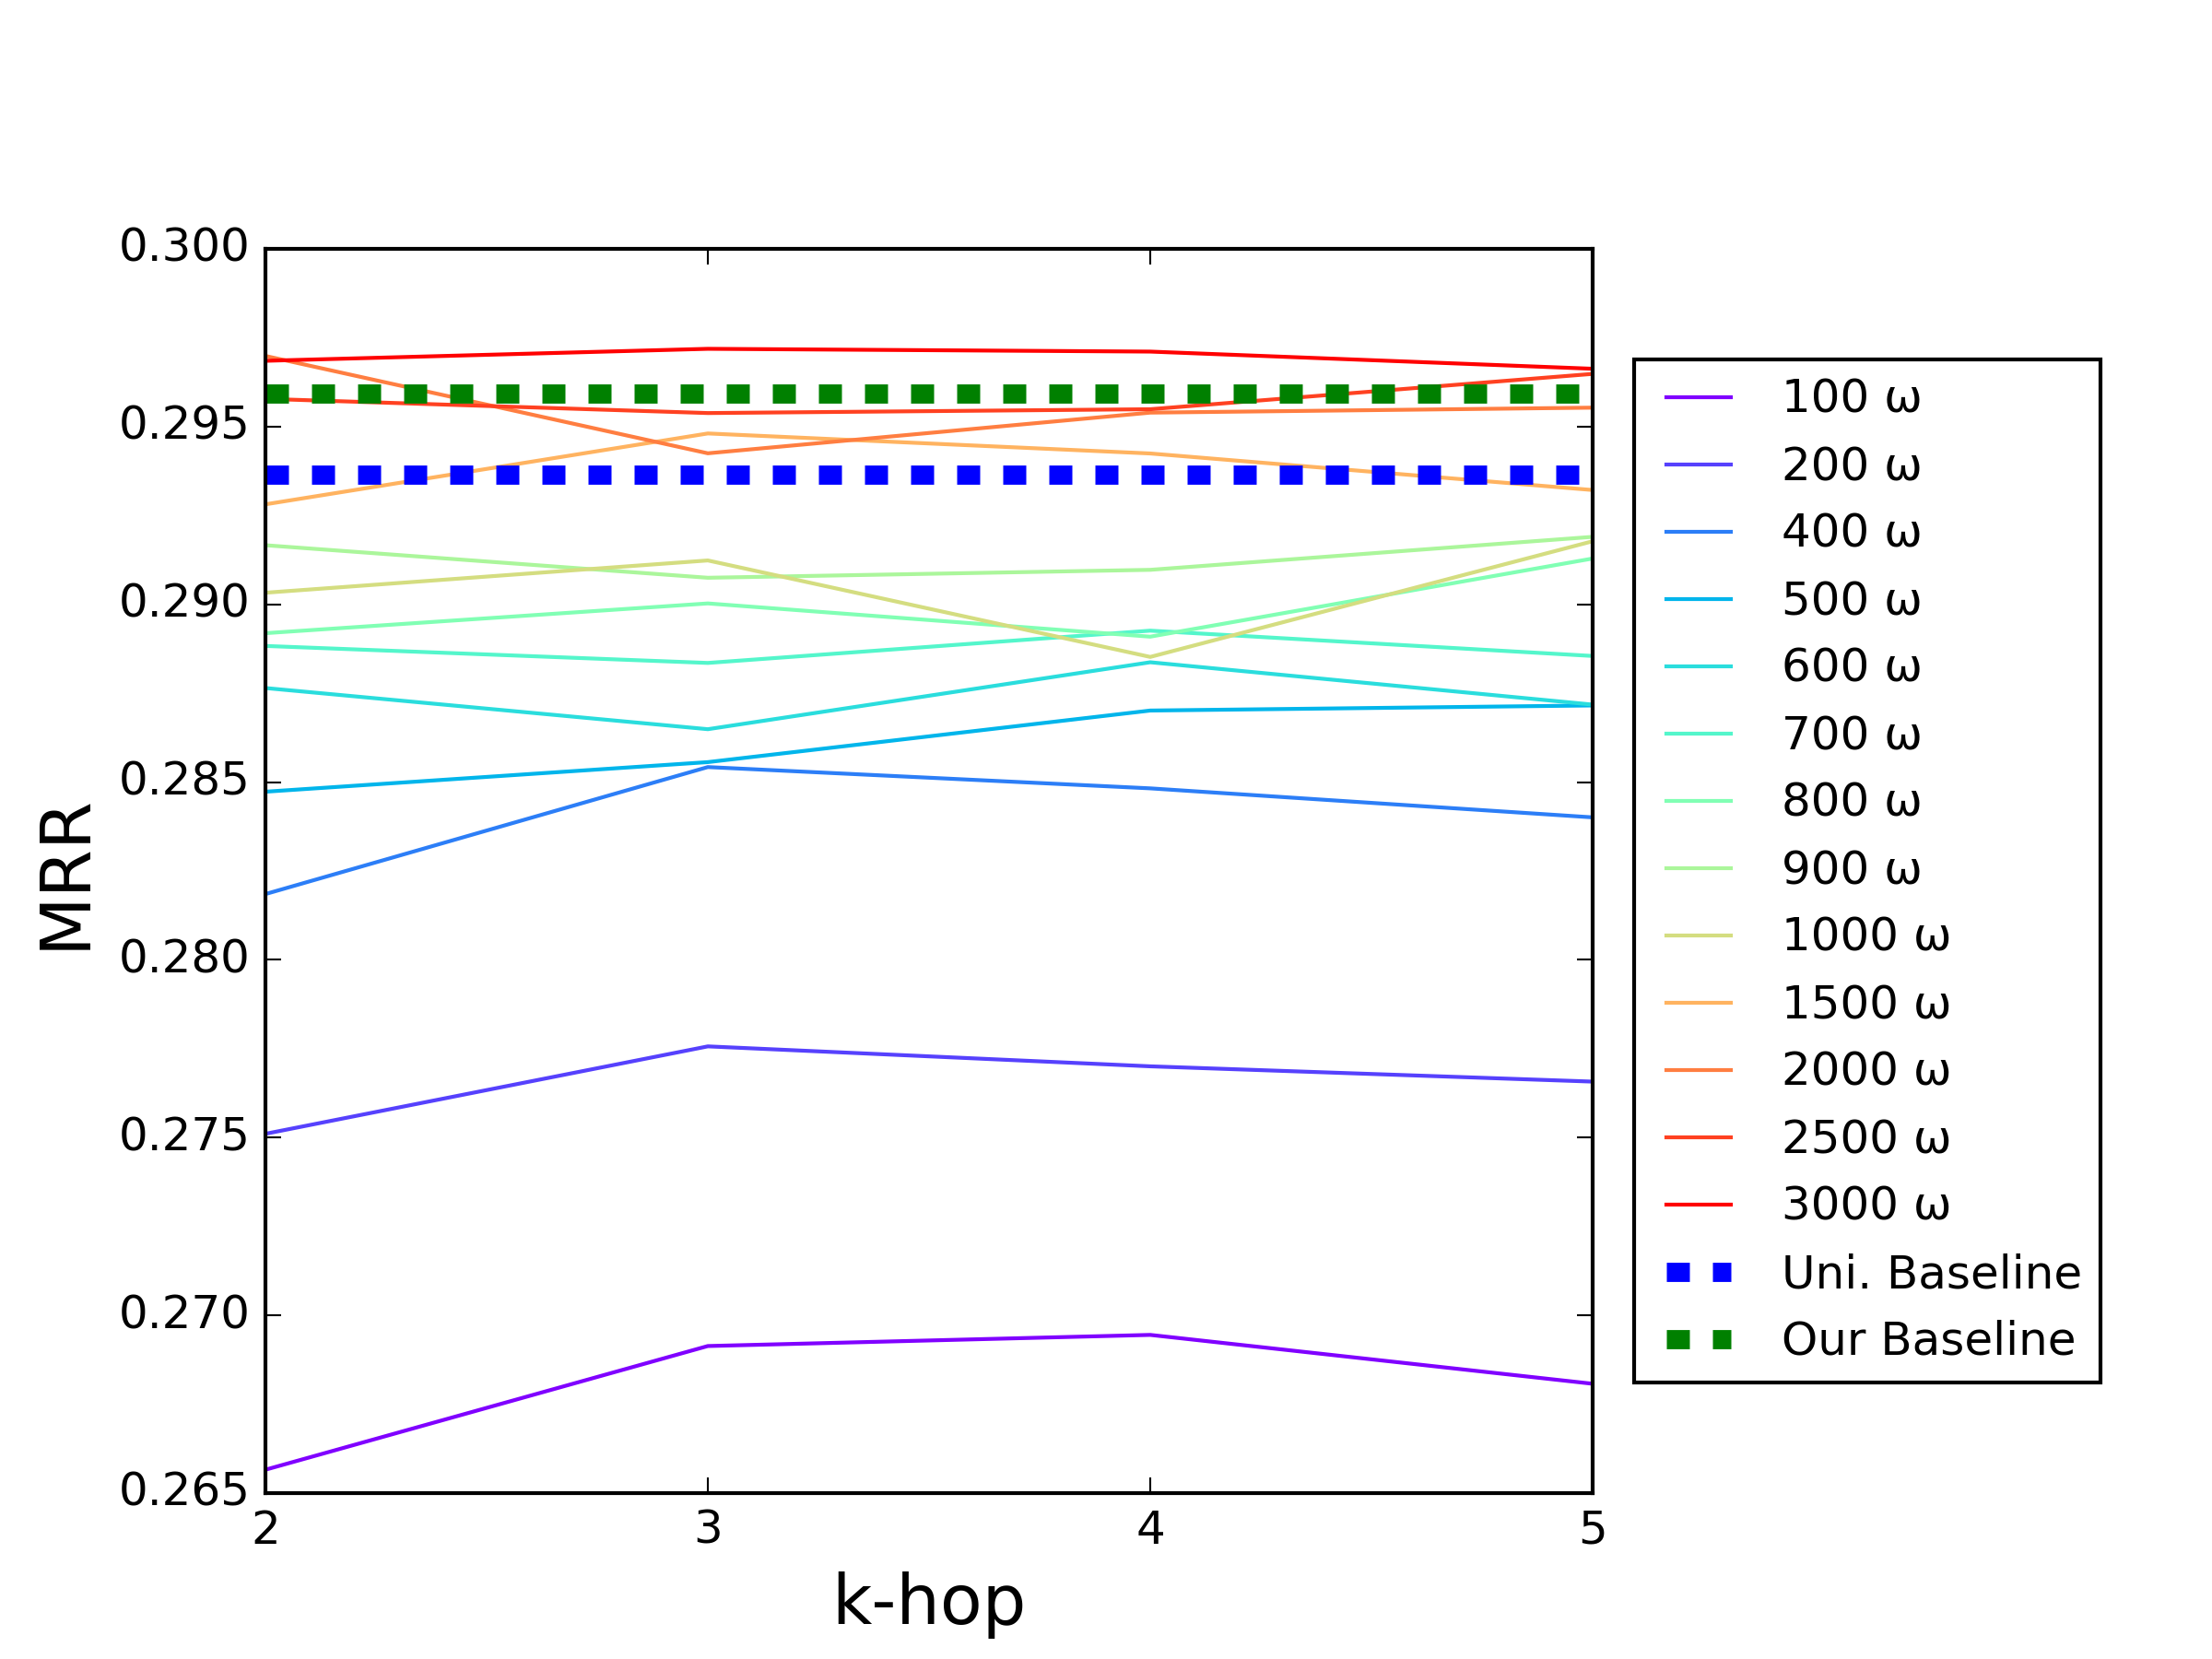
\includegraphics[width=2.5in]{writeup/Results/Ablation.png}
    \caption{The effect of the number of random walks
     for Uniform SANS with the TransE on FB 15k-237.}
    \label{fig:ablation}
\end{figure}

% END OF RESULTS
% ---------------------------------------------------------------

\cut{
Table \ref{tab:unisota_comp} compares the performance of uniform SANS negative sampling with state of the art algorithms, used to train different graph embedding models on different datasets. As indicated, not only uniform SANS beats uniform negative sampling in FB15K-237, it almost always outperforms it in the WN18 dataset, only losing to it marginally.  This out-performance is especially significant when uniform SANS is fused with TransE and DistMult, where an increase of 0.2143 and 0.2864 in MRR is noticed respectively. Comparing Uniform SANS with other negative sampling approaches, SANS beats KBGAN in all experimental setups except for one. Additionally, it beats NSCaching when used to train TransE. This finding re-iterates the ``hardness'' of negative examples that lie in the \emph{k-hop} neighbourhood of the nodes, as NSCaching works by caching and sampling from high quality negative triplets.} 

\cut{
On the other hand, Table \ref{tab:comp_adv} is indicative of the performance of Self-Adversarial negative sampling against our Self-Adversarial SANS. As noted, Self-Adversarial SANS beats Self-Adversarial on FB15K-237 and WN18 when fused with DisMult, while achieves close performance to it in other settings. By acknowledging the similarity in their performance and the nature of the distribution of negative samples used in Self-Adversarial SANS, the importance of local negatives when training graph embedding models is emphasized, supporting our hypothesis. This observation further implies the computational feasibility of our approach compared to Self-Adversarial, for using a smaller distribution of negative triplets. \cut{, as listed in Table \ref{tab:percentage}.}}

\cut{Lastly, Table \ref{tab:comp_sota} compares the performance of uniform SANS with some of the state-of-the-arts. As seen, uniform SANS beats KBGAN in all experimental setups except for one. Additionally, it beats NSCaching when used to train TransE. This finding re-iterates the ``hardness'' of negative examples that lie in the \emph{k-hop} neighbourhood of the nodes, as NSCaching works by caching and sampling from high quality negative triplets.} 

\cut{To infer the number of random walks which can adequately approximate the k-hop tensor, we investigated the effect of different numbers of random walks, $\omega$, ranging from 100 to 3000 illustrated in Figure \ref{fig:ablation}. In these graphs, two baselines are exhibited, namely the one representing the output when negative sampling was done uniformly, and the other being our best performance achieved by our Uniform SANS combined with TransE, for which the k-hop tensor was explicitly computed. According to our observations, our model beats both baselines when the k-hop tensor is approximated with 3000 random walks. This result can be justified by acknowledging that the nodes’ indices that are within close proximity in the k-hop tensor will have larger values; this will yield a weighted negative sampling scheme and may be the contributor to the increased performance.}







